\section{Where actor--critic fits: the RL road to equilibrium, and its potholes}\label{sec:rl}

\mkey{why ppo self-play fails}A reader arriving from applied RL asks the obvious question: why not just PPO in self-play --- policy network, value critic, reward = chips, train against a copy of yourself? The answer is a theorem, not a tuning problem. Perolat et al.~\cite{perolat2020} proved that the idealized dynamics of gradient self-play in two-player zero-sum imperfect-information games are \emph{Poincar\'e-recurrent}: trajectories \textbf{orbit} the equilibrium and return arbitrarily close to where they started, forever. The learning vector field \emph{rotates} around the solution instead of pointing at it (Figure~\ref{fig:cycle}, left) --- rock--paper--scissors chasing, at scale, in your GPU bill. \pitfall{Cycling in zero-sum self-play is geometry, not a hyperparameter problem: no learning-rate schedule fixes a field with no attraction.} The deep reason is Section~\ref{sec:solving}'s fact 2: equilibria are \emph{mixed}, and ``improve greedily against the current opponent'' has no mixed fixed point to settle into.

\begin{figure}[t]
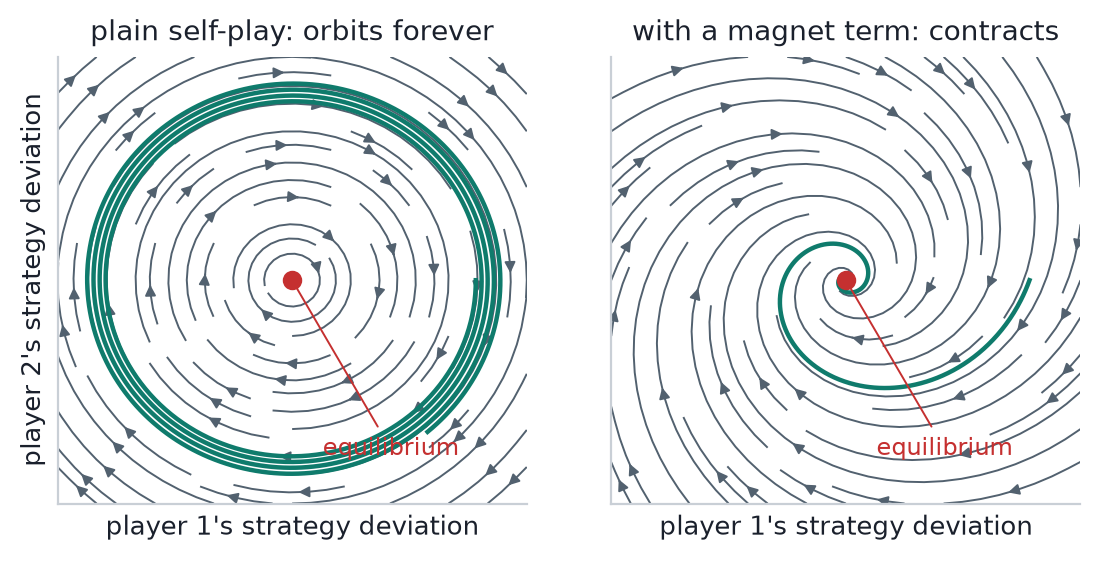
\includegraphics[width=\linewidth]{figures/cycle.png}
\caption{Real trajectories of the two dynamics (simulated for this paper): unregularized self-play orbits; adding a KL pull toward a reference policy makes the same dynamics contract.}
\label{fig:cycle}
\end{figure}

Contrast the games where naive self-play \emph{does} work --- AlphaZero's chess, shogi, Go~\cite{alphazero}. Perfect information supplies two pillars: every state has a minimax value independent of beliefs (so a value target exists), and a deterministic optimal policy exists (so greedy improvement is a genuine ladder). Hidden cards demolish both --- values depend on ranges, ranges on both strategies, and optimal play must randomize. Everything that works in imperfect information restores convergence by one of three escapes:

\begin{center}
\footnotesize
\begin{tabular}{@{}p{0.62in}p{1.02in}p{2.86in}@{}}
\toprule
Escape & Method & Mechanism, and its cost \\
\midrule
\textbf{Average} & NFSP (2016)~\cite{nfsp} & DQN best-responds to the opponent's \emph{historical average} policy; a supervised net learns that average and is what you deploy. Cost: slow; beaten by Deep CFR. \\
\textbf{Population} & PSRO (2017)~\cite{psro} & meta-game over whole trained policies: solve the small matrix, train a new RL best response to the mixture, repeat. Cost: a full RL run per iteration; coarse at poker's fine mixing. \\
\textbf{Regularize} & R-NaD / DeepNash (2022)~\cite{deepnash}; MMD (2023)~\cite{mmd} & add a KL pull toward a reference ``magnet'' policy --- the regularized game has a \emph{unique} equilibrium the dynamics contract to; move the magnet, repeat. Cost: a regularization schedule; guarantees soften under sampling. \\
\bottomrule
\end{tabular}
\end{center}

The averaging escape should feel familiar: it is CFR's own trick wearing RL clothes (fictitious play averages policies; CFR averages in regret space). The regularization escape is the modern one --- DeepNash reached top-3 human ranking in \emph{Stratego} ($10^{535}$ nodes) model-free, no search, and its ``last-iterate'' property means the final network itself is the answer, no averaging machinery. MMD is its minimal form --- mirror descent plus one extra KL term, the first standard-RL-shaped algorithm empirically competitive with tabular CFR on benchmark games --- and the honest note is that its deep-RL evidence so far is small games. \mnote{If the project ever wants an RL baseline next to Deep CFR: tabular MMD drops into the same Kuhn/Leduc harness as one extra loss term --- the version of ``PPO self-play'' that has a convergence story.}

\subsection*{The honesty file: what PPO actually does in poker}

\mkey{alphaholdem}The strongest published PPO-style result is \textbf{AlphaHoldem} (2022~\cite{alphaholdem}): Trinal-Clip PPO (an extra ratio clip when advantages are negative, plus pot-bounded value targets) and a K-best pool of historical selves, trained three days on one PC --- beat Slumbot by 111\,mbb/hand and pros by 10\,mbb/hand, deciding in 3\,ms. Tempting. The catch is what head-to-head wins cannot certify: in the Approximate Exploitability study~\cite{timbers2022}, two bots statistically \emph{indistinguishable} head-to-head differed by $\sim$1{,}300\,mbb/hand in measured exploitability. \hlight{Head-to-head strength and closeness-to-equilibrium are different quantities, and only the second is a solver's claim} --- for Drawmaha, where no external opponent exists to even run the head-to-head, a PPO bot's quality would be simply unmeasurable. There is also a mechanical reason PPO underperforms here, found only recently~\cite{vrpo}: GAE's advantage estimates carry variance from sampling your own future actions, and because equilibrium play is \emph{deliberately} stochastic, that variance persists even with a perfect critic --- expected-SARSA-style traces (VRPO) are the drop-in fix. File both away for the day the project trains its planned PPO baseline.

So where does actor--critic \emph{legitimately} live in this project? Three places, all supporting roles: as the \textbf{exploiter} --- train a PPO/DQN best response against the \emph{frozen} final network, where the opponent holds still, cycling vanishes, and the exploiter's winnings are an exploitability lower bound (Section~\ref{sec:evaluation}); as \textbf{baselines} inside variance-reduced MCCFR, which are control-variate critics by another name (Section~\ref{sec:mccfr}); and as the parked \textbf{comparison chapter} --- CFR solution vs.\ PPO self-play agent, with the exploiter quantifying the gap the theory predicts.
